\documentclass[xcolor=pdftex,svgnames,table]{beamer}
\usepackage{latexsym,amssymb,amsmath,stmaryrd}
\usepackage[utf8]{inputenc}
\usepackage[T1]{fontenc}
\usepackage[francais]{babel}
\usepackage{pgf}
\usepackage{tikz}
\usetikzlibrary{arrows,patterns,plotmarks,shapes,snakes,er,3d,automata,%
backgrounds,topaths,trees,petri,mindmap}
\usepackage{pgfbaseimage}
\usepackage{ifpdf}
\ifpdf
\usepackage{graphicx}
\else
%\usepackage[dvips]{graphicx}
\usepackage{pstricks,pst-tree,pst-node}
\newpsobject{showgrid}{psgrid}{subgriddiv=1,griddots=10,gridlabels=6pt}
\fi
\usepackage{moreverb}
\usepackage[normalem]{ulem}
\usepackage{version}
\usepackage{url}
\usepackage{multicol}
\usepackage{listings}
\lstset{
  language=[ANSI]C, 
%  gobble=2, 
%  escapeinside="", 
  basicstyle=\ttfamily, 
%  directivestyle=\color{Fuchsia},
  identifierstyle = \color{DarkOrange},
  keywordstyle=\color{DarkGreen}, 
  commentstyle=\color{red}, 
%  numbers=left, 
%  numbersep=5pt, 
%  numberstyle=\scriptsize, 
%  moredelim=[is][\color{gray}\itshape]{/*}{*/}, 
%  moredelim=[is][\alert]{/+}{+/}, 
%  morecomment=[is]{/=}{=/}, 
%  morecomment=[in]{comment=}{,} 
%  fancyvrb=true 
} 

\newcommand{\binaire}[1]{\ensuremath{\underline{#1}}}
\newcommand{\C}[1]{\texttt{#1}}
\newcommand{\bbbn}{\ensuremath{\mathbb{N}}}
%%%%%%%%%%%%%%%%%%%%%%%%%%%%%%%%%%%%%%%%%%%%%%%%%%%%%%%%%%%%%%%%
%% ccBeamer 0.1, 2007-07-02                                   %%
%% Written by Sebastian Pipping <webmaster@hartwork.org>      %%
%% ---------------------------------------------------------- %%
%% Licensed under Creative Commons Attribution-ShareAlike 3.0 %%
%% http://creativecommons.org/licenses/by-sa/3.0/             %%
%%%%%%%%%%%%%%%%%%%%%%%%%%%%%%%%%%%%%%%%%%%%%%%%%%%%%%%%%%%%%%%%


%% Images
\newcommand{\CcImageBy}[1]{%
	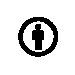
\includegraphics[scale=#1]{creative_commons/cc_by_30}%
}
\newcommand{\CcImageCc}[1]{%
	
\includegraphics[scale=#1]{creative_commons/cc_cc_30}%
}
\newcommand{\CcImageDevNations}[1]{%
	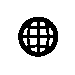
\includegraphics[scale=#1]{creative_commons/cc_dev_nations_30}%
}
\newcommand{\CcImageNc}[1]{%
	
\includegraphics[scale=#1]{creative_commons/cc_nc_30}%
}
\newcommand{\CcImageNd}[1]{%
	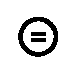
\includegraphics[scale=#1]{creative_commons/cc_nd_30}%
}
\newcommand{\CcImagePd}[1]{%
	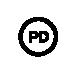
\includegraphics[scale=#1]{creative_commons/cc_pd_30}%
}
\newcommand{\CcImageSa}[1]{%
	
\includegraphics[scale=#1]{creative_commons/cc_sa_30}%
}
\newcommand{\CcImageSampling}[1]{%
	
\includegraphics[scale=#1]{creative_commons/cc_sampling_30}%
}
\newcommand{\CcImageSamplingPlus}[1]{%
	
\includegraphics[scale=#1]{creative_commons/cc_sampling_plus_30}%
}


%% Groups
\newcommand{\CcGroupBy}[1]{% zoom
	\CcImageBy{#1}%
}
\newcommand{\CcGroupByNc}[2]{% zoom, gap
	\CcImageBy{#1}\hspace*{#2}\CcImageNc{#1}%
}
\newcommand{\CcGroupByNcNd}[2]{% zoom, gap
	\CcImageBy{#1}\hspace*{#2}\CcImageNc{#1}\hspace*{#2}\CcImageNd{#1}%
}
\newcommand{\CcGroupByNcSa}[2]{% zoom, gap
	\CcImageBy{#1}\hspace*{#2}\CcImageNc{#1}\hspace*{#2}\CcImageSa{#1}%
}
\newcommand{\CcGroupByNd}[2]{% zoom, gap
	\CcImageBy{#1}\hspace*{#2}\CcImageNd{#1}%
}
\newcommand{\CcGroupBySa}[2]{% zoom, gap
	\CcImageBy{#1}\hspace*{#2}\CcImageSa{#1}%
}
\newcommand{\CcGroupDevNations}[1]{% zoom
	\CcImageDevNations{#1}%
}
\newcommand{\CcGroupNcSampling}[2]{% zoom, gap
	\CcImageNc{#1}\hspace*{#2}\CcImageSampling{#1}%
}
\newcommand{\CcGroupPd}[1]{% zoom
	\CcImagePd{#1}%
}
\newcommand{\CcGroupSampling}[1]{% zoom
	\CcImageSampling{#1}%
}
\newcommand{\CcGroupSamplingPlus}[1]{% zoom
	\CcImageSamplingPlus{#1}%
}


%% Text
\newcommand{\CcLongnameBy}{Attribution}
\newcommand{\CcLongnameByNc}{Attribution-NonCommercial}
\newcommand{\CcLongnameByNcNd}{Attribution-NoDerivs}
\newcommand{\CcLongnameByNcSa}{Attribution-NonCommercial-ShareAlike}
\newcommand{\CcLongnameByNd}{Attribution-NoDerivs}
\newcommand{\CcLongnameBySa}{Attribution-ShareAlike}

\newcommand{\CcNote}[1]{% longname
	This work is licensed under the \textit{Creative Commons #1 3.0 License}.%
}

\usetheme{classic}
\newcommand{\nowrite}{\put(10,-4){\includegraphics[scale=.05]{creative_commons/nopencil}}}
\newcommand{\youwrite}{\put(10,-4){
\includegraphics[scale=.05]{creative_commons/pencil}}}
\newcommand{\writethat}{
\includegraphics[scale=.05]{creative_commons/pencil}}
\newcommand{\aemporter}{\put(10,-6){
\includegraphics[scale=.05]{creative_commons/szymonraj_Shopping_bag}}}


%%% Titre -- cours 10
\title{Éléments d'informatique -- Cours 10.\\ Types composés: structures (enregistrements)}
\author{Pierre Boudes}
\date{\today}

\begin{document}

%% Page de titre et licence CC.
\begin{frame}
	\titlepage
	\vfill
	\begin{center}
		\CcGroupByNcSa{0.83}{0.95ex}\\[2.5ex]
		{\tiny\CcNote{\CcLongnameByNcSa}}
		\vspace*{-2.5ex}
	\end{center}
\end{frame}


%%%%%%%%%%%%%%%%%%%%



 \section*{Contenu du cours}
\begin{frame}
%  \frametitle{Contenu du cours (rappel)}
 \begin{itemize}
  \item \emph{Éléments d'architecture des ordinateurs (+mini-assembleur)}\nowrite
  \item \emph{Éléments de systèmes d'exploitation}
\item Programmation structurée impérative (éléments de langage C)
\begin{itemize}
  \item \emph{Structure d'un programme C}
  \item \emph{Variables : déclaration (et initialisation), affectaction}
  \item \emph{Évaluation d'expressions}
  \item \emph{Instructions de contrôle : if, for, while}
  \item \emph{Types de données : entiers, caractères,
    réels}, \emph{tableaux}, enregistrements
  \item \emph{Fonctions d'entrées/sorties (scanf/printf)}
  \item \emph{Écriture et appel de fonctions}
  \item Débogage
\end{itemize}
\item \emph{Notions de compilation
  \begin{itemize}
  \item Analyse lexicale, analyse syntaxique, analyse sémantique
  \item préprocesseur du compilateur C (include, define)
   \item Édition de lien
  \end{itemize}}
\item Algorithmes élémentaires
\item Méthodologie de résolution, manipulation sous linux
\end{itemize}
\end{frame}


\section[Plan]{}
\frame[label=plan]{\frametitle{Plan de la séance\nowrite}\tableofcontents}


\section[Introduction]{Introduction}
\begin{frame}
  \frametitle{Introduction}
\pause
Les données déclarées comme
ayant un type de base (int, double, char) ne contiennent qu'un seule
valeur. Tandis qu'une donnée de type structure \alert{englobe plusieurs
  valeurs}.\pause
\begin{itemize}
\item Une structure s'utilise comme un \alert{type}. \pause
\item Chacune des valeurs est accessible à l'aide d'un nom, fixé à la
  déclaration de la structure. On parle des \alert{champs} de la
  structure.\pause
\item Un type structure doit être déclaré avant d'être
  utilisé. Ne pas confondre : \textbf{déclaration de variable} (dans une
  fonction) et \textbf{déclaration de type structure} ou  \textbf{déclaration de fonction}.
\pause
\item Les valeurs des champs d'une variable (d'un type structure donné)
  peuvent être accédées et modifiées individuellement à l'aide de la
  \alert{notation pointée}. \pause
\item On peut aussi manipuler globalement la valeur d'une donnée de
  type structure. Par exemple : faire une affectation entre variables
  d'un même type structure (copie de tous les champs).
\end{itemize}
\end{frame}

\section[Déclaration]{Déclaration d'un type utilisateur struct}
\begin{frame}[fragile]
  \frametitle{Déclaration d'un type utilisateur struct}
Comme avec les variables, comme avec les fonctions, avant de pouvoir
utiliser un type structure, il faut déclarer son nom
(convention: suffixe \verb|_s|), et la liste de ses
champs sous la forme \verb|type nom_champ;|
\pause
\begin{lstlisting}[escapechar={\%},basicstyle=\ttfamily\small] 
struct bulletin_s 
{
  double temperature; /* temperature de l'air */
  int force;          /* force du vent (Beaufort) */
}; /* <-- attention ';' (cas particulier) */
\end{lstlisting}
\pause
\begin{itemize}
\item Cette déclaration est placée en dehors de toute fonction, entre
les définitions de constantes symboliques (\verb|#define ...|) et les
déclarations de fonctions utilisateur.
\pause
\item L'effet de cette déclaration est de signaler au compilateur qu'un nouveau
type est disponible et comment il peut être utilisé (liste des champs). Aucun espace mémoire n'est réservé à ce moment
(ce n'est pas une déclaration de variable).
\item \pause \alert{Attention au point-vigule final}.
\end{itemize}
\end{frame}

\section[Utilisation]{Utilisation d'un type utilisateur struct}
\begin{frame}[fragile]
  \frametitle{Utilisation d'un type utilisateur struct: variables}

\begin{lstlisting}[escapechar={\%},basicstyle=\ttfamily\small] 
int main()
{
    struct bulletin_s x = {0.5, 4};
    struct bulletin_s y;
    
    y = x; /* copie globale */
    x.temperature = 13.4; /* modif. d'un champ */
    ...
}
\end{lstlisting}
\pause
\begin{itemize}
\item Initialisation:  syntaxe proche de celle des tableaux.
\pause
\item la déclaration d'une variable de type structure reprend le mot
  clé \verb|struct| et le nom donné à la structure.
\pause
\item On accéde aux éléments d'une structure à l'aide de la notation
  pointée :
\verb|nom_variable.nom_champ|
\end{itemize}
\end{frame}

%\section{Type utilisateur struct et fonctions (utilisateur)}
\begin{frame}[fragile]
  \frametitle{Utilisation d'un type utilisateur struct: fonctions}

\begin{lstlisting}[escapechar={\%},basicstyle=\ttfamily\small] 
/* declaration de fonctions utilisateur */
struct bm_s moyenne_bm(struct bm_s x, struct bm_s y);
\end{lstlisting}
\pause
On emploie \verb|struct nom_struct|, comme pour une déclaration de variable.
\begin{lstlisting}[escapechar={\%},basicstyle=\ttfamily\small] 

/* definitions des fonctions utilisateur */
struct bm_s moyenne_bm(struct bm_s x, struct bm_s y)
{
    struct bm_s nouveau_bm;

    nouveau_bm.temperature = (x.temperature 
                              + y.temperature) / 2.0;
    nouveau_bm.force = (x.force + y.force) / 2;

    return nouveau_bm;
}
\end{lstlisting}
\end{frame}

\section[trace]{Traces avec type utilisateur structure}
\begin{frame}[fragile]
  \frametitle{Traces avec type utilisateur structure}
{
\rowcolors{2}{green!50}{yellow!50} %\arrayrulecolor{green!75!gray}
\small
      \setlength{\unitlength}{\tabcolsep}
        \begin{tabular}[t]{|r|c|c|c|c|c|c|l|}
          \multicolumn{8}{l}{\C{moyenne\_bm(\{14.1, 2\}, \{9.5,
              4\})}}\\ \hline
\rowcolor{green!50}
          ligne & \multicolumn{2}{>{\columncolor{green!50}}c|}{x} 
                & \multicolumn{2}{>{\columncolor{green!50}}c|}{y} & \multicolumn{2}{>{\columncolor{green!50}}c|}{nouveau\_bm} & A. \\ \hline
             & temperature & force & temperature & force & temperature & force &  \\ \hline
          ini.  & 14.1 & 2 & 9.5 & 4 & ? & ? & \\ \hline
          40  & & & & & 11.8 &  & \\ \hline
          42  & & & & &  & 3 & \\ \hline
        44 &\multicolumn{7}{>{\columncolor{green!50}}l}{RETOURNE \{11.8, 3\}}\\ \hline
        \end{tabular}
}
\end{frame}

\section[Intérêt]{Intérêt des structures (enregistrements)}
\begin{frame}
  \frametitle{Intérêt des structures (enregistrements)}

Intérêt des structures  :
  \begin{itemize}
   \item \structure{lisibilité} : regrouper un ensemble
      de données dans un même type, nommé de façon explicite,
      facilite la relecture du code;\pause
  \item \structure{augmente les possibilités} : les structures permettent d'écrire des
    fonctions qui retournent plusieurs valeurs, en l'absence de pointeurs.\pause
    \item \structure{modularité} : on peut rajouter des champs très
      facilement, avec très peu de modifications.\pause
    \item \structure{Incontournables :} les langages orientés objets
      généralisent la notion de structure. Un objet est une structure
      dont les champs peuvent être aussi bien des données que des
      fonctions (hors programme).
  \end{itemize}
\end{frame}

\section[Quelques erreurs]{Quelques erreurs communes}
\begin{frame}[fragile]
  \frametitle{Erreurs communes}

\begin{itemize}
\item Message d'erreur \emph{étrange} :
\begin{lstlisting}[numbers=left,basicstyle=\ttfamily\small,firstnumber=7] 
struct bm_s 
{
  double temperature; /* temperature de l'air */
  int force;          /* force du vent (Beaufort) */
}

/* Declaration des fonctions utilisateur */
void afficher_bm(struct bm_s);
\end{lstlisting}
{\small
\begin{verbatim}
14: error: two or more data types in declaration specifiers
\end{verbatim}
}
\pause
\alert{Oubli du point-virgule !}
\pause
\item Champ inexistant :
\begin{lstlisting}[numbers=left,basicstyle=\ttfamily\small,firstnumber=22] 
    x.toto = 3; /* erreur: pas de champs toto */
\end{lstlisting}
{\small
\begin{verbatim}
prog.c: In function ‘main’:
prog.c:22: error: ‘struct bm_s’ has no member named ‘toto’
\end{verbatim}
}
\end{itemize}
\end{frame}

\end{document}

% revenir sur :
%-l'appel au cours suivant : paramètre et expression, pile d'appel.
%-la grammaire des identificateurs